\documentclass[11pt]{article}
\usepackage{amsmath}
\usepackage{amssymb}
\usepackage{graphicx}
\usepackage{tabularx}
\usepackage{fancyhdr}
\usepackage{lastpage}

% Page layout
\usepackage[top=1in, bottom=1in, left=1in, right=1in]{geometry}

% Header and footer
\pagestyle{fancy}
\fancyhf{}
\rfoot{Page \thepage}
\renewcommand{\headrulewidth}{0pt}

% Modified Question command with left-aligned number
\newcommand{\questiona}[2]{
    \noindent\textbf{Q#2.} #1 \hfill \textbf{[1 Mark]}
}

\newcommand{\questionb}[2]{
    \noindent\textbf{Q#2.} #1 \hfill \textbf{[2 Marks]}
}

\begin{document}

% Title section with horizontal line
\begin{center}
    \Large\textbf{GATE 2018 - Physics (PH)} \\
    \large\textbf{General Aptitude and Technical Questions} \\
    \rule{\textwidth}{0.5pt} % Horizontal line below heading
\end{center}

\vspace{0.5cm}

% General Aptitude Section
\section*{General Aptitude}

\questiona{``When she fell down the \_\_\_\_\_, she received many \_\_\_\_\_ but little help.''}{1}
\begin{enumerate}
    \item[(A)] stairs, stares  
    \item[(B)] stairs, stairs  
    \item[(C)] stares, stairs  
    \item[(D)] stares, stares  
\end{enumerate}
\vspace{0.5cm}

\questiona{``In spite of being warned repeatedly, he failed to correct his \_\_\_\_\_ behaviour.''}{2}
\begin{enumerate}
    \item[(A)] rational  
    \item[(B)] reasonable  
    \item[(C)] errant  
    \item[(D)] good  
\end{enumerate}
\vspace{0.5cm}

\questiona{For \(0 \leq x \leq 2\pi\), \(\sin x\) and \(\cos x\) are both decreasing functions in the interval \_\_\_\_\_.}{3}
\begin{enumerate}
    \item[(A)] \((0, \frac{\pi}{2})\)  
    \item[(B)] \((\frac{\pi}{2}, \pi)\)  
    \item[(C)] \((\pi, \frac{3\pi}{2})\)  
    \item[(D)] \((\frac{3\pi}{2}, 2\pi)\)  
\end{enumerate}
\vspace{0.5cm}

\questiona{The area of an equilateral triangle is \(\sqrt{3}\). What is the perimeter of the triangle?}{4}
\begin{enumerate}
    \item[(A)] 2  
    \item[(B)] 4  
    \item[(C)] 6  
    \item[(D)] 8  
\end{enumerate}
\vspace{0.5cm}

\questiona{Arrange the following three-dimensional objects in the descending order of their volumes: (i) A cuboid with dimensions 10 cm, 8 cm and 6 cm, (ii) A cube of side 8 cm, (iii) A cylinder with base radius 7 cm and height 7 cm, (iv) A sphere of radius 7 cm}{5}
\begin{enumerate}
    \item[(A)] (i), (ii), (iii), (iv)  
    \item[(B)] (ii), (i), (iv), (iii)  
    \item[(C)] (iii), (ii), (i), (iv)  
    \item[(D)] (iv), (iii), (ii), (i)  
\end{enumerate}
\vspace{0.5cm}

\questionb{An automobile travels from city A to city B and returns to city A by the same route. The speed of the vehicle during the onward and return journeys were constant at 60 km/h and 90 km/h, respectively. What is the average speed in km/h for the entire journey?}{6}
\begin{enumerate}
    \item[(A)] 72  
    \item[(B)] 73  
    \item[(C)] 74  
    \item[(D)] 75  
\end{enumerate}
\vspace{0.5cm}

\questionb{A set of 4 parallel lines intersect with another set of 5 parallel lines. How many parallelograms are formed?}{7}
\begin{enumerate}
    \item[(A)] 20  
    \item[(B)] 48  
    \item[(C)] 60  
    \item[(D)] 72  
\end{enumerate}
\vspace{0.5cm}

\questionb{To pass a test, a candidate needs to answer at least 2 out of 3 questions correctly. A total of 6,30,000 candidates appeared for the test. Question A was correctly answered by 3,30,000 candidates. Question B by 2,50,000 candidates. Question C by 2,60,000 candidates. A and B both by 1,00,000. B and C by 90,000. A and C by 80,000. If the number answering all questions is the same as the number answering none, how many failed to clear the test?}{8}
\begin{enumerate}
    \item[(A)] 30,000  
    \item[(B)] 2,70,000  
    \item[(C)] 3,90,000  
    \item[(D)] 4,20,000  
\end{enumerate}
\vspace{0.5cm}

\questionb{If \(x^2 + x - 1 = 0\), what is the value of \(x^4 + \frac{1}{x^4}\)?}{9}
\begin{enumerate}
    \item[(A)] 1  
    \item[(B)] 5  
    \item[(C)] 7  
    \item[(D)] 9  
\end{enumerate}
\vspace{0.5cm}

\questionb{In a detailed study of annual crow births in India, it was found there was relatively no growth during 2002–2004 and a sudden spike from 2004 to 2005. In an unrelated study, revenue from cracker sales remained flat from 2002–2004, but spiked in 2005 before declining in 2006. The solid line in the graph below refers to annual sale of crackers and the dashed line refers to the annual crow births in India. Choose the most appropriate inference.}{10}
\begin{center}
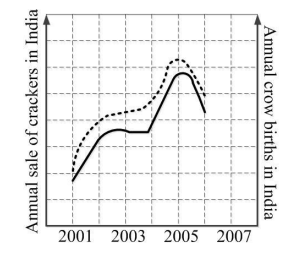
\includegraphics[width=0.5\textwidth]{figures/10.png}
\end{center}
\begin{enumerate}
    \item[(A)] There is a strong correlation between crow birth and cracker sales.  
    \item[(B)] Cracker usage increases crow birth rate.  
    \item[(C)] If cracker sale declines, crow birth will decline.  
    \item[(D)] Increased birth rate of crows will cause an increase in the sale of crackers.  
\end{enumerate}
\vspace{0.5cm}

\section*{Technical Section}

\questiona{The eigenvalues of a Hermitian matrix are all}{1}
\begin{enumerate}
    \item[(A)] real  
    \item[(B)] imaginary  
    \item[(C)] of modulus one  
    \item[(D)] real and positive  
\end{enumerate}
\vspace{0.5cm}

\questiona{Which one of the following represents the 3p radial wave function of hydrogen atom? (a\textsubscript{0} is the Bohr radius)}{2}
\begin{center}
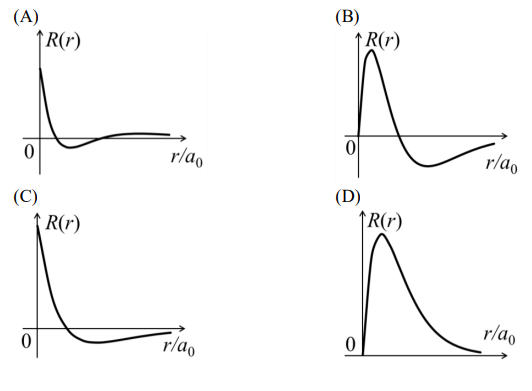
\includegraphics[width=0.8\textwidth]{figures/2.png}
\end{center}
\vspace{0.5cm}

\questiona{Given the following table, match Group I with Group II: 

\begin{tabular}{ll}
P: Stern-Gerlach experiment & 1: Wave nature of particles \\
Q: Zeeman effect & 2: Quantization of energy of electrons in atoms \\
R: Frank-Hertz experiment & 3: Existence of electron spin \\
S: Davisson-Germer experiment & 4: Space quantization of angular momentum \\
\end{tabular}

Which one of the following correctly matches the experiments?}{3}
\begin{enumerate}
    \item[(A)] P-2, Q-3, R-4, S-1  
    \item[(B)] P-1, Q-3, R-2, S-4  
    \item[(C)] P-3, Q-4, R-2, S-1  
    \item[(D)] P-2, Q-1, R-4, S-3  
\end{enumerate}
\vspace{0.5cm}

\questiona{In spherical polar coordinates \((r, \theta, \phi)\), the unit vector \(\hat{\theta}\) at \((10, \frac{\pi}{4}, \frac{\pi}{2})\) is}{4}
\begin{enumerate}
    \item[(A)] \(\hat{z}\)  
    \item[(B)] \(\frac{1}{\sqrt{2}}(\hat{j} + \hat{z})\)  
    \item[(C)] \(\frac{1}{\sqrt{2}}(-\hat{j} + \hat{z})\)  
    \item[(D)] \(\frac{1}{\sqrt{2}}(\hat{j} - \hat{z})\)  
\end{enumerate}
\vspace{0.5cm}

\questiona{The scale factors corresponding to the covariant metric tensor \(g_{ij}\) in spherical polar coordinates are}{5}
\begin{enumerate}
    \item[(A)] 1, \(r^2\), \(r^2 \sin^2 \theta\)  
    \item[(B)] 1, \(r^2\), \(\sin^2 \theta\)  
    \item[(C)] 1, 1, 1  
    \item[(D)] 1, \(r\), \(r \sin \theta\)  
\end{enumerate}
\vspace{0.5cm}

\questiona{In the context of small oscillations, which one of the following does NOT apply to the normal coordinates?}{6}
\begin{enumerate}
    \item[(A)] Each normal coordinate has an eigen-frequency associated with it  
    \item[(B)] The normal coordinates are orthogonal to one another  
    \item[(C)] The normal coordinates are all independent  
    \item[(D)] The potential energy of the system is a sum of squares of the normal coordinates with constant coefficients  
\end{enumerate}
\vspace{0.5cm}

\questiona{For the given unit cells of a two-dimensional square lattice, which option lists all the primitive cells?}{7}
\begin{center}
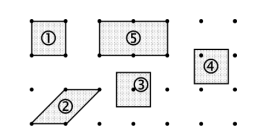
\includegraphics[width=0.5\textwidth]{figures/7.png}
\end{center}
\begin{enumerate}
    \item[(A)] 1 and 2  
    \item[(B)] 1, 2 and 3 
    \item[(C)] 1, 2, 3 and 4 
    \item[(D)] 1, 2, 3, 4 and 5  
\end{enumerate}
\vspace{0.5cm}

\questiona{Among electric field (\(\vec{E}\)), magnetic field (\(\vec{B}\)), angular momentum (\(\vec{L}\)), and vector potential (\(\vec{A}\)), which is/are odd under parity (space inversion) operation?}{8}
\begin{enumerate}
    \item[(A)] \(\vec{E}\) only  
    \item[(B)] \(\vec{E}\) and \(\vec{A}\) only  
    \item[(C)] \(\vec{E}\) and \(\vec{L}\) only  
    \item[(D)] \(\vec{B}\) and \(\vec{L}\) only  
\end{enumerate}
\vspace{0.5cm}

\questiona{The expression for the second overtone frequency in the vibrational absorption spectra of a diatomic molecule in terms of the harmonic frequency \(\omega_e\) and anharmonicity constant \(x_e\) is}{9}
\begin{enumerate}
    \item[(A)] \(2\omega_e(1 - x_e)\)  
    \item[(B)] \(2\omega_e(1 - 3x_e)\)  
    \item[(C)] \(3\omega_e(1 - 2x_e)\)  
    \item[(D)] \(3\omega_e(1 - 4x_e)\)  
\end{enumerate}
\vspace{0.5cm}

\questiona{Match the physical effects and order of magnitude of their energy scales below, where \(\alpha = \frac{e^2}{4\pi\epsilon_0\hbar c}\) is the fine structure constant; \(m_e\) and \(m_p\) are electron and proton masses, respectively:

\begin{tabular}{ll}
P: Lamb shift & 1: \(\sim \mathcal{O}(\alpha^2 m_e c^2)\) \\
Q: Fine structure & 2: \(\sim \mathcal{O}(\alpha^4 m_e c^2)\) \\
R: Bohr energy & 3: \(\sim \mathcal{O}(\alpha^4 m_e^2 c^2 / m_p)\) \\
S: Hyperfine structure & 4: \(\sim \mathcal{O}(\alpha^5 m_e c^2)\) \\
\end{tabular}}{10}
\begin{enumerate}
    \item[(A)] P-3, Q-1, R-2, S-4  
    \item[(B)] P-2, Q-3, R-1, S-4  
    \item[(C)] P-4, Q-2, R-1, S-3  
    \item[(D)] P-2, Q-4, R-1, S-3  
\end{enumerate}
\vspace{0.5cm}

\questiona{The logic expression \(\overline{A}BC + \overline{A}\overline{B}C + AB\overline{C} + A\overline{B}\overline{C}\) can be simplified to}{11}
\begin{enumerate}
    \item[(A)] \(A \oplus C\)  
    \item[(B)] \(A \land \overline{C}\)  
    \item[(C)] 0  
    \item[(D)] 1  
\end{enumerate}
\vspace{0.5cm}

\questiona{At low temperatures (T), the specific heat of common metals is described by (with \(\alpha\) and \(\beta\) as constants)}{12}
\begin{enumerate}
    \item[(A)] \(\alpha T + \beta T^3\)  
    \item[(B)] \(\beta T^3\)  
    \item[(C)] \(\exp(-\alpha/T)\)  
    \item[(D)] \(\alpha T + \beta T^5\)  
\end{enumerate}
\vspace{0.5cm}

\questiona{In a 2-to-1 multiplexer as shown below, the output \(X = A_0\) if \(C = 0\), and \(X = A_1\) if \(C = 1\). }{13}
\begin{center}
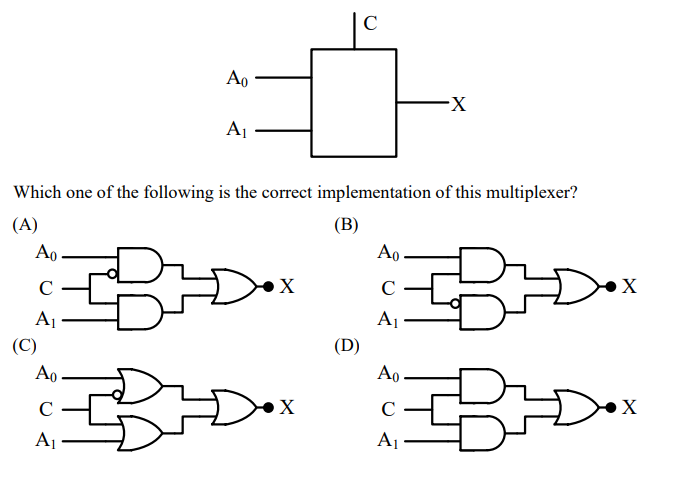
\includegraphics[width=1\textwidth]{figures/13.png}
\end{center}

\vspace{0.5cm}

\questiona{The elementary particle \(\Xi^0\) is placed in the baryon decuplet shown below at}{14}
\begin{center}
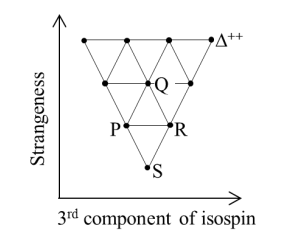
\includegraphics[width=0.5\textwidth]{figures/14.png}
\end{center}
\begin{enumerate}
    \item[(A)] P  
    \item[(B)] Q  
    \item[(C)] R  
    \item[(D)] S  
\end{enumerate}
\vspace{0.5cm}

\questiona{The intrinsic/permanent electric dipole moment in the ground state of hydrogen atom is (\(a_0\) is the Bohr radius)}{15}
\begin{enumerate}
    \item[(A)] \(-3ea_0\)  
    \item[(B)] zero  
    \item[(C)] \(ea_0\)  
    \item[(D)] \(3ea_0\)  
\end{enumerate}
\vspace{0.5cm}

\questiona{The high temperature magnetic susceptibility of solids having ions with magnetic moments can be described by \(\chi \propto \frac{1}{T + \theta}\) with T as absolute temperature and \(\theta\) as constant. The three behaviors i.e. paramagnetic, ferromagnetic and antiferromagnetic are described, respectively, by}{16}
\begin{enumerate}
    \item[(A)] \(\theta < 0\), \(\theta > 0\), \(\theta = 0\)  
    \item[(B)] \(\theta > 0\), \(\theta < 0\), \(\theta = 0\)  
    \item[(C)] \(\theta = 0\), \(\theta < 0\), \(\theta > 0\)  
    \item[(D)] \(\theta = 0\), \(\theta > 0\), \(\theta < 0\)  
\end{enumerate}
\vspace{0.5cm}

\questiona{Which one of the following is an allowed electric dipole transition?}{17}
\begin{enumerate}
    \item[(A)] \(1S_0 \rightarrow 3S_1\)  
    \item[(B)] \(2P_{3/2} \rightarrow 2D_{5/2}\)  
    \item[(C)] \(2D_{5/2} \rightarrow 2P_{1/2}\)  
    \item[(D)] \(3P_0 \rightarrow 5D_0\)  
\end{enumerate}
\vspace{0.5cm}

\questiona{In the decay, \(\mu^+ \rightarrow e^+ + \nu_e + X\), what is X?}{18}
\begin{enumerate}
    \item[(A)] \(\gamma\)  
    \item[(B)] \(\bar{\nu}_e\)  
    \item[(C)] \(\nu_{\mu}\)  
    \item[(D)] \(\bar{\nu}_{\mu}\)  
\end{enumerate}
\vspace{0.5cm}

\questiona{A spaceship is travelling with a velocity of \(0.7c\) away from a space station. The spaceship ejects a probe with a velocity \(0.59c\) opposite to its own velocity. A person in the space station would see the probe moving at a speed \(Xc\), where the value of \(X\) is \_\_\_\_\_ (up to three decimal places).}{19}
\vspace{0.5cm}

\questiona{For an operational amplifier (ideal) circuit shown below, if \(V_1 = 1\text{ V}\) and \(V_2 = 2\text{ V}\), the value of \(V_0\) is \_\_\_\_\_ V (up to one decimal place).}{20}
\begin{center}
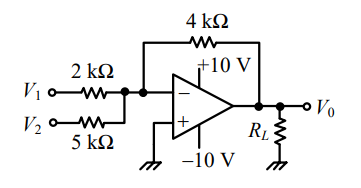
\includegraphics[width=0.5\textwidth]{figures/20.png}
\end{center}
\vspace{0.5cm}

\questiona{An infinitely long straight wire is carrying a steady current \(I\). The ratio of magnetic energy density at distance \(r_1\) to that at \(r_2 (= 2r_1)\) from the wire is \_\_\_\_\_.}{21}
\vspace{0.5cm}

\questiona{A light beam of intensity \(I_0\) is falling normally on a surface. The surface absorbs 20\% of the intensity and the rest is reflected. The radiation pressure on the surface is given by \(X I_0 / c\), where \(X =\) \_\_\_\_\_ (up to one decimal place).}{22}
\vspace{0.5cm}

\questiona{The number of independent components of a general electromagnetic field tensor is \_\_\_\_\_.}{23}
\vspace{0.5cm}

\questiona{If \(X\) is the dimensionality of a free electron gas, the energy (\(E\)) dependence of density of states is given by \(E^{\frac{1}{2}X - Y}\), where \(Y =\) \_\_\_\_\_.}{24}
\vspace{0.5cm}

\questiona{For nucleus \({}^{164}\text{Er}\), a \(J^\pi = 2^+\) state is at 90 keV. Assuming \({}^{164}\text{Er}\) to be a rigid rotor, the energy of its \(4^+\) state is \_\_\_\_\_ keV (up to one decimal place).}{25}
\vspace{0.5cm}

\questionb{Given \(\vec{v}_1 = \hat{i} - \hat{j}\) and \(\vec{v}_2 = -2\hat{i} + 3\hat{j} + 2\hat{k}\), which one of the following \(\vec{v}_3\) makes \((\vec{v}_1, \vec{v}_2, \vec{v}_3)\) a complete set for a three dimensional real linear vector space?}{26}
\begin{enumerate}
    \item[(A)] \(\vec{v}_3 = \hat{i} + \hat{j} + 4\hat{k}\)  
    \item[(B)] \(\vec{v}_3 = 2\hat{i} - \hat{j} + 2\hat{k}\)  
    \item[(C)] \(\vec{v}_3 = \hat{i} + 2\hat{j} + 6\hat{k}\)  
    \item[(D)] \(\vec{v}_3 = 2\hat{i} + \hat{j} + 4\hat{k}\)  
\end{enumerate}
\vspace{0.5cm}

\questionb{An interstellar object has speed \(v\) at the point of its shortest distance \(R\) from a star of much larger mass \(M\). Given \(v^2 = \frac{2GM}{R}\), the trajectory of the object is}{27}
\begin{enumerate}
    \item[(A)] circle  
    \item[(B)] ellipse  
    \item[(C)] parabola  
    \item[(D)] hyperbola  
\end{enumerate}
\vspace{0.5cm}

\questionb{A particle moves in one dimension under a potential \(V(x) = \alpha |x|\) with some non-zero total energy. Which one of the following best describes the particle trajectory in the phase space?}{28}
\begin{center}
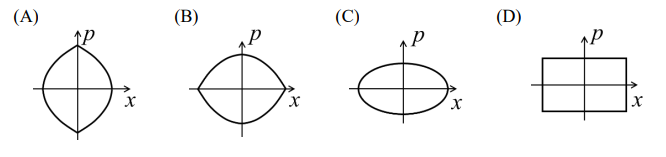
\includegraphics[width=0.9\textwidth]{figures/28.png}
\end{center}
\vspace{0.5cm}

\questionb{Consider an infinitely long solenoid with \(N\) turns per unit length, radius \(R\) and carrying a current \(I(t) = \alpha \cos(\omega t)\), where \(\alpha\) is a constant and \(\omega\) is the angular frequency. The magnitude of electric field at the surface of the solenoid is}{29}
\begin{enumerate}
    \item[(A)] \(\frac{1}{2} \mu_0 N R \omega \alpha \sin(\omega t)\)  
    \item[(B)] \(\frac{1}{2} \mu_0 \omega N R \cos(\omega t)\)  
    \item[(C)] \(\mu_0 N R \omega \alpha \sin(\omega t)\)  
    \item[(D)] \(\mu_0 \omega N R \cos(\omega t)\)  
\end{enumerate}
\vspace{0.5cm}

\questionb{A constant and uniform magnetic field \(\vec{B} = B_0 \hat{z}\) pervades all space. Which one of the following is the correct choice for the vector potential in Coulomb gauge?}{30}
\begin{enumerate}
    \item[(A)] \(-B_0(x + y)\hat{i}\)  
    \item[(B)] \(B_0(x + y)\hat{j}\)  
    \item[(C)] \(B_0 x \hat{j}\)  
    \item[(D)] \(-\frac{1}{2}B_0(x\hat{i} - y\hat{j})\)  
\end{enumerate}
\vspace{0.5cm}

\questionb{If \(H\) is the Hamiltonian for a free particle with mass \(m\), the commutator \([x, [x, H]]\) is}{31}
\begin{enumerate}
    \item[(A)] \(\frac{\hbar^2}{m}\)  
    \item[(B)] \(-\frac{\hbar^2}{m}\)  
    \item[(C)] \(-\frac{\hbar^2}{2m}\)  
    \item[(D)] \(\frac{\hbar^2}{2m}\)  
\end{enumerate}
\vspace{0.5cm}

\questionb{A long straight wire, having radius \(a\) and resistance per unit length \(r\), carries a current \(I\). The magnitude and direction of the Poynting vector on the surface of the wire is}{32}
\begin{enumerate}
    \item[(A)] \(\frac{I^2 r}{2\pi a}\), perpendicular to axis of the wire and pointing inwards  
    \item[(B)] \(\frac{I^2 r}{2\pi a}\), perpendicular to axis of the wire and pointing outwards  
    \item[(C)] \(\frac{I^2 r}{\pi a}\), perpendicular to axis of the wire and pointing inwards  
    \item[(D)] \(\frac{I^2 r}{\pi a}\), perpendicular to axis of the wire and pointing outwards  
\end{enumerate}
\vspace{0.5cm}

\questionb{Three particles are to be distributed in four non-degenerate energy levels. The possible number of ways of distribution: (i) for distinguishable particles, and (ii) for identical Bosons, respectively, is}{33}
\begin{enumerate}
    \item[(A)] (i) 24, (ii) 4  
    \item[(B)] (i) 24, (ii) 20  
    \item[(C)] (i) 64, (ii) 20  
    \item[(D)] (i) 64, (ii) 16  
\end{enumerate}
\vspace{0.5cm}

\questionb{The term symbol for the electronic ground state of oxygen atom is}{34}
\begin{enumerate}
    \item[(A)] \(^1S_0\)  
    \item[(B)] \(^1D_2\)  
    \item[(C)] \(^3P_0\)  
    \item[(D)] \(^3P_2\)  
\end{enumerate}
\vspace{0.5cm}

\questionb{The energy dispersion for electrons in one-dimensional lattice with lattice parameter \(a\) is given by \(E(k) = E_0 - \frac{1}{2} W \cos(ka)\), where \(W\) and \(E_0\) are constants. The effective mass of the electron near the bottom of the band is}{35}
\begin{enumerate}
    \item[(A)] \(\frac{2\hbar^2}{W a^2}\)  
    \item[(B)] \(\frac{\hbar^2}{W a^2}\)  
    \item[(C)] \(\frac{\hbar^2}{2W a^2}\)  
    \item[(D)] \(\frac{\hbar^2}{4W a^2}\)  
\end{enumerate}
\vspace{0.5cm}

\questionb{Amongst electrical resistivity (\(\rho\)), thermal conductivity (\(\kappa\)), specific heat (\(C\)), Young’s modulus (\(Y\)), and magnetic susceptibility (\(\chi\)), which quantities show a sharp change at the superconducting transition temperature?}{36}
\begin{enumerate}
    \item[(A)] \(\rho, \kappa, C, Y\)  
    \item[(B)] \(\rho, C, \chi\)  
    \item[(C)] \(\rho, \kappa, C, \chi\)  
    \item[(D)] \(\kappa, Y, \chi\)  
\end{enumerate}
\vspace{0.5cm}

\questionb{A quarter wave plate introduces a path difference of \(\lambda/4\) between the two components of polarization parallel and perpendicular to the optic axis. An electromagnetic wave with \(\vec{E} = (\hat{i} + \hat{j}) E_0 e^{i(kz - \omega t)}\) is incident normally on a quarter wave plate which has its optic axis making an angle \(135^\circ\) with the x-axis as shown. The emergent electromagnetic wave would be}{37}
\begin{center}
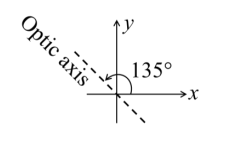
\includegraphics[width=0.5\textwidth]{figures/37.png}
\end{center}
\begin{enumerate}
    \item[(A)] elliptically polarized  
    \item[(B)] circularly polarized  
    \item[(C)] linearly polarized with polarization as that of incident wave  
    \item[(D)] linearly polarized but with polarization at \(90^\circ\) to that of the incident wave  
\end{enumerate}
\vspace{0.5cm}

\questionb{A p-doped semiconductor slab carries a current \(I = 100\) mA in a magnetic field \(B = 0.2\) T as shown. One measures \(V_y = 0.25\) mV and \(V_x = 2\) mV. The mobility of holes in the semiconductor is \_\_\_\_\_ m\(^2\)V\(^{-1}\)s\(^{-1}\) (up to two decimal places).}{38}
\begin{center}
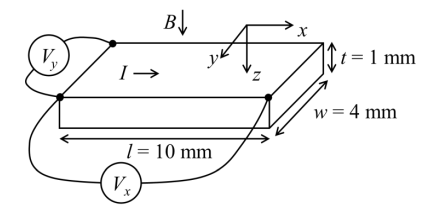
\includegraphics[width=0.5\textwidth]{figures/38.png}
\end{center}
\vspace{0.5cm}

\questionb{An n-channel FET having Gate-Source switch-off voltage \(V_{GS(\text{OFF})} = -2\) V is used to invert a 0 – 5 V square-wave signal as shown. The maximum allowed value of \(R\) would be \_\_\_\_\_ k\(\Omega\) (up to two decimal places).}{39}
\begin{center}
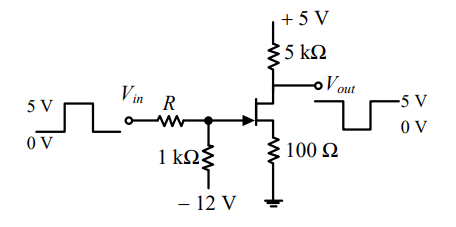
\includegraphics[width=0.5\textwidth]{figures/39.png}
\end{center}
\vspace{0.5cm}

\questionb{Inside a large nucleus, a nucleon with mass 939 MeV/\(c^2\) has Fermi momentum 1.40 fm\(^{-1}\) at absolute zero temperature. Its velocity is \(Xc\), where the value of \(X\) is \_\_\_\_\_ (up to two decimal places).}{40}
\vspace{0.5cm}

\questionb{4 MeV \(\gamma\)-rays emitted by the de-excitation of \({}^{19}\text{F}\) are attributed, assuming spherical symmetry, to the transition of protons from \(1d_{3/2}\) state to \(1d_{5/2}\) state. If the contribution of spin-orbit term to the total energy is written as \(C \langle \vec{l} \cdot \vec{s} \rangle\), the magnitude of \(C\) is \_\_\_\_\_ MeV (up to one decimal place).}{41}
\vspace{0.5cm}

\questionb{An \(\alpha\)-particle is emitted by a \({}^{230}_{90}\text{Th}\) nucleus. Assuming the potential to be purely Coulombic beyond the point of separation, the height of the Coulomb barrier is \_\_\_\_\_ MeV (up to two decimal places).\\
(\(\frac{e^2}{4\pi\epsilon_0} = 1.44\) MeV·fm, \(r_0 = 1.30\) fm)}{42}
\vspace{0.5cm}

\questionb{For the transformation \(Q = \sqrt{2q} e^{-1 + 2\alpha} \cos p\), \(P = \sqrt{2q} e^{-\alpha - 1} \sin p\), (where \(\alpha\) is a constant) to be canonical, the value of \(\alpha\) is \_\_\_\_\_.}{43}
\vspace{0.5cm}

\questionb{Given \(\frac{d^2f(x)}{dx^2} - 2\frac{df(x)}{dx} + f(x) = 0\), and boundary conditions \(f(0) = 1\) and \(f(1) = 0\), the value of \(f(0.5)\) is \_\_\_\_\_ (up to two decimal places).}{44}
\vspace{0.5cm}

\questionb{The absolute value of the integral \(\int \frac{5z^3 + 3z^2}{z^2 - 4} dz\), over the circle \(|z - 1.5| = 1\) in complex plane, is \_\_\_\_\_ (up to two decimal places).}{45}
\vspace{0.5cm}

\questionb{A uniform circular disc of mass \(m\) and radius \(R\) is rotating with angular speed \(\omega\) about an axis passing through its center and making an angle \(\theta = 30^\circ\) with the axis of the disc. If the kinetic energy of the disc is \(\alpha m \omega^2 R^2\), the value of \(\alpha\) is \_\_\_\_\_ (up to two decimal places).}{46}
\begin{center}
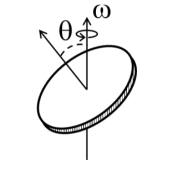
\includegraphics[width=0.5\textwidth]{figures/46.png}
\end{center}
\vspace{0.5cm}

\questionb{The ground state energy of a particle of mass \(m\) in an infinite potential well is \(E_0\). It changes to \(E_0(1 + \alpha \times 10^{-3})\), when there is a small potential bump of height \(V_0 = \frac{\pi^2 \hbar^2}{50mL^2}\) and width \(a = L/100\). The value of \(\alpha\) is \_\_\_\_\_ (up to two decimal places).}{47}
\begin{center}
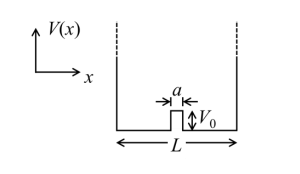
\includegraphics[width=0.5\textwidth]{figures/47.png}
\end{center}
\vspace{0.5cm}

\questionb{An electromagnetic plane wave is propagating with an intensity \(I = 1.0 \times 10^5\) Wm\(^{-2}\) in a medium with \(\epsilon = 3\epsilon_0\) and \(\mu = \mu_0\). The amplitude of the electric field inside the medium is \_\_\_\_\_ × \(10^3\) Vm\(^{-1}\) (up to one decimal place). \\
(\(\epsilon_0 = 8.85 \times 10^{-12}\) C\(^2\)/N·m\(^2\), \(\mu_0 = 4\pi \times 10^{-7}\) N/A\(^2\), \(c = 3 \times 10^8\) m/s)}{48}
\vspace{0.5cm}

\questionb{A microcanonical ensemble consists of 12 atoms with each taking either energy 0 state, or energy \(\epsilon\) state. Both states are non-degenerate. If the total energy of this ensemble is \(4\epsilon\), its entropy will be \_\_\_\_\_ \(k_B\) (up to one decimal place), where \(k_B\) is the Boltzmann constant.}{49}
\vspace{0.5cm}

\questionb{A two-state quantum system has energy eigenvalues \(\pm \epsilon\) corresponding to the normalized states \(|\psi_\pm\rangle\). At time \(t = 0\), the system is in quantum state \(\frac{1}{\sqrt{2}}[|\psi_+\rangle + |\psi_-\rangle]\). The probability that the system will be in the same state at \(t = \frac{h}{6\epsilon}\) is \_\_\_\_\_ (up to two decimal places).}{50}
\vspace{0.5cm}

\questionb{An air-conditioner maintains the room temperature at \(27^\circ\text{C}\) while the outside temperature is \(47^\circ\text{C}\). The heat conducted through the walls of the room from outside to inside due to temperature difference is 7000 W. The minimum work done by the compressor of the air-conditioner per unit time is \_\_\_\_\_ W.}{51}
\vspace{0.5cm}

\questionb{Two solid spheres A and B have same emissivity. The radius of A is four times the radius of B, and temperature of A is twice the temperature of B. The ratio of the rate of heat radiated from A to that from B is \_\_\_\_\_.}{52}
\vspace{0.5cm}

\questionb{The partition function of an ensemble at a temperature \(T\) is \(Z = (2 \cosh(\frac{\epsilon}{k_BT}))^N\), where \(k_B\) is the Boltzmann constant. The heat capacity of this ensemble at \(T = \frac{\epsilon}{k_B}\) is \(X N k_B\), where the value of \(X\) is \_\_\_\_\_ (up to two decimal places).}{53}
\vspace{0.5cm}

\questionb{An atom in its singlet state is subjected to a magnetic field. The Zeeman splitting of its 650 nm spectral line is 0.03 nm. The magnitude of the field is \_\_\_\_\_ Tesla (up to two decimal places). \\
(\(e = 1.60 \times 10^{-19}\) C, \(m_e = 9.11 \times 10^{-31}\) kg, \(c = 3.0 \times 10^8\) m/s)}{54}
\vspace{0.5cm}

\questionb{The quantum effects in an ideal gas become important below a certain temperature \(T_Q\) when de Broglie wavelength corresponding to the root mean square thermal speed becomes equal to the inter-atomic separation. For such a gas of atoms of mass \(2 \times 10^{-26}\) kg and number density \(6.4 \times 10^{25}\) m\(^{-3}\), \(T_Q =\) \_\_\_\_\_ × \(10^{-3}\) K (up to one decimal place). \\
(\(k_B = 1.38 \times 10^{-23}\) J/K, \(h = 6.6 \times 10^{-34}\) J·s)}{55}
\vspace{0.5cm}

\vspace{5cm}
\begin{center}
\textbf{END OF THE QUESTION PAPER}\\
\rule{\textwidth}{0.5pt}
\end{center}

\end{document}
